% Generated by Sphinx.
\def\sphinxdocclass{report}
\documentclass[letterpaper,10pt,english]{sphinxmanual}
\usepackage[utf8]{inputenc}
\DeclareUnicodeCharacter{00A0}{\nobreakspace}
\usepackage{cmap}
\usepackage[T1]{fontenc}
\usepackage{babel}
\usepackage{times}
\usepackage[Bjarne]{fncychap}
\usepackage{longtable}
\usepackage{sphinx}
\usepackage{multirow}

\addto\captionsenglish{\renewcommand{\figurename}{Fig. }}
\addto\captionsenglish{\renewcommand{\tablename}{Table }}
\floatname{literal-block}{Listing }



\title{Nukestar Documentation}
\date{September 24, 2015}
\release{0.1}
\author{william gurecky}
\newcommand{\sphinxlogo}{}
\renewcommand{\releasename}{Release}
\makeindex

\makeatletter
\def\PYG@reset{\let\PYG@it=\relax \let\PYG@bf=\relax%
    \let\PYG@ul=\relax \let\PYG@tc=\relax%
    \let\PYG@bc=\relax \let\PYG@ff=\relax}
\def\PYG@tok#1{\csname PYG@tok@#1\endcsname}
\def\PYG@toks#1+{\ifx\relax#1\empty\else%
    \PYG@tok{#1}\expandafter\PYG@toks\fi}
\def\PYG@do#1{\PYG@bc{\PYG@tc{\PYG@ul{%
    \PYG@it{\PYG@bf{\PYG@ff{#1}}}}}}}
\def\PYG#1#2{\PYG@reset\PYG@toks#1+\relax+\PYG@do{#2}}

\expandafter\def\csname PYG@tok@gd\endcsname{\def\PYG@tc##1{\textcolor[rgb]{0.63,0.00,0.00}{##1}}}
\expandafter\def\csname PYG@tok@gu\endcsname{\let\PYG@bf=\textbf\def\PYG@tc##1{\textcolor[rgb]{0.50,0.00,0.50}{##1}}}
\expandafter\def\csname PYG@tok@gt\endcsname{\def\PYG@tc##1{\textcolor[rgb]{0.00,0.27,0.87}{##1}}}
\expandafter\def\csname PYG@tok@gs\endcsname{\let\PYG@bf=\textbf}
\expandafter\def\csname PYG@tok@gr\endcsname{\def\PYG@tc##1{\textcolor[rgb]{1.00,0.00,0.00}{##1}}}
\expandafter\def\csname PYG@tok@cm\endcsname{\let\PYG@it=\textit\def\PYG@tc##1{\textcolor[rgb]{0.25,0.50,0.56}{##1}}}
\expandafter\def\csname PYG@tok@vg\endcsname{\def\PYG@tc##1{\textcolor[rgb]{0.73,0.38,0.84}{##1}}}
\expandafter\def\csname PYG@tok@m\endcsname{\def\PYG@tc##1{\textcolor[rgb]{0.13,0.50,0.31}{##1}}}
\expandafter\def\csname PYG@tok@mh\endcsname{\def\PYG@tc##1{\textcolor[rgb]{0.13,0.50,0.31}{##1}}}
\expandafter\def\csname PYG@tok@cs\endcsname{\def\PYG@tc##1{\textcolor[rgb]{0.25,0.50,0.56}{##1}}\def\PYG@bc##1{\setlength{\fboxsep}{0pt}\colorbox[rgb]{1.00,0.94,0.94}{\strut ##1}}}
\expandafter\def\csname PYG@tok@ge\endcsname{\let\PYG@it=\textit}
\expandafter\def\csname PYG@tok@vc\endcsname{\def\PYG@tc##1{\textcolor[rgb]{0.73,0.38,0.84}{##1}}}
\expandafter\def\csname PYG@tok@il\endcsname{\def\PYG@tc##1{\textcolor[rgb]{0.13,0.50,0.31}{##1}}}
\expandafter\def\csname PYG@tok@go\endcsname{\def\PYG@tc##1{\textcolor[rgb]{0.20,0.20,0.20}{##1}}}
\expandafter\def\csname PYG@tok@cp\endcsname{\def\PYG@tc##1{\textcolor[rgb]{0.00,0.44,0.13}{##1}}}
\expandafter\def\csname PYG@tok@gi\endcsname{\def\PYG@tc##1{\textcolor[rgb]{0.00,0.63,0.00}{##1}}}
\expandafter\def\csname PYG@tok@gh\endcsname{\let\PYG@bf=\textbf\def\PYG@tc##1{\textcolor[rgb]{0.00,0.00,0.50}{##1}}}
\expandafter\def\csname PYG@tok@ni\endcsname{\let\PYG@bf=\textbf\def\PYG@tc##1{\textcolor[rgb]{0.84,0.33,0.22}{##1}}}
\expandafter\def\csname PYG@tok@nl\endcsname{\let\PYG@bf=\textbf\def\PYG@tc##1{\textcolor[rgb]{0.00,0.13,0.44}{##1}}}
\expandafter\def\csname PYG@tok@nn\endcsname{\let\PYG@bf=\textbf\def\PYG@tc##1{\textcolor[rgb]{0.05,0.52,0.71}{##1}}}
\expandafter\def\csname PYG@tok@no\endcsname{\def\PYG@tc##1{\textcolor[rgb]{0.38,0.68,0.84}{##1}}}
\expandafter\def\csname PYG@tok@na\endcsname{\def\PYG@tc##1{\textcolor[rgb]{0.25,0.44,0.63}{##1}}}
\expandafter\def\csname PYG@tok@nb\endcsname{\def\PYG@tc##1{\textcolor[rgb]{0.00,0.44,0.13}{##1}}}
\expandafter\def\csname PYG@tok@nc\endcsname{\let\PYG@bf=\textbf\def\PYG@tc##1{\textcolor[rgb]{0.05,0.52,0.71}{##1}}}
\expandafter\def\csname PYG@tok@nd\endcsname{\let\PYG@bf=\textbf\def\PYG@tc##1{\textcolor[rgb]{0.33,0.33,0.33}{##1}}}
\expandafter\def\csname PYG@tok@ne\endcsname{\def\PYG@tc##1{\textcolor[rgb]{0.00,0.44,0.13}{##1}}}
\expandafter\def\csname PYG@tok@nf\endcsname{\def\PYG@tc##1{\textcolor[rgb]{0.02,0.16,0.49}{##1}}}
\expandafter\def\csname PYG@tok@si\endcsname{\let\PYG@it=\textit\def\PYG@tc##1{\textcolor[rgb]{0.44,0.63,0.82}{##1}}}
\expandafter\def\csname PYG@tok@s2\endcsname{\def\PYG@tc##1{\textcolor[rgb]{0.25,0.44,0.63}{##1}}}
\expandafter\def\csname PYG@tok@vi\endcsname{\def\PYG@tc##1{\textcolor[rgb]{0.73,0.38,0.84}{##1}}}
\expandafter\def\csname PYG@tok@nt\endcsname{\let\PYG@bf=\textbf\def\PYG@tc##1{\textcolor[rgb]{0.02,0.16,0.45}{##1}}}
\expandafter\def\csname PYG@tok@nv\endcsname{\def\PYG@tc##1{\textcolor[rgb]{0.73,0.38,0.84}{##1}}}
\expandafter\def\csname PYG@tok@s1\endcsname{\def\PYG@tc##1{\textcolor[rgb]{0.25,0.44,0.63}{##1}}}
\expandafter\def\csname PYG@tok@gp\endcsname{\let\PYG@bf=\textbf\def\PYG@tc##1{\textcolor[rgb]{0.78,0.36,0.04}{##1}}}
\expandafter\def\csname PYG@tok@sh\endcsname{\def\PYG@tc##1{\textcolor[rgb]{0.25,0.44,0.63}{##1}}}
\expandafter\def\csname PYG@tok@ow\endcsname{\let\PYG@bf=\textbf\def\PYG@tc##1{\textcolor[rgb]{0.00,0.44,0.13}{##1}}}
\expandafter\def\csname PYG@tok@sx\endcsname{\def\PYG@tc##1{\textcolor[rgb]{0.78,0.36,0.04}{##1}}}
\expandafter\def\csname PYG@tok@bp\endcsname{\def\PYG@tc##1{\textcolor[rgb]{0.00,0.44,0.13}{##1}}}
\expandafter\def\csname PYG@tok@c1\endcsname{\let\PYG@it=\textit\def\PYG@tc##1{\textcolor[rgb]{0.25,0.50,0.56}{##1}}}
\expandafter\def\csname PYG@tok@kc\endcsname{\let\PYG@bf=\textbf\def\PYG@tc##1{\textcolor[rgb]{0.00,0.44,0.13}{##1}}}
\expandafter\def\csname PYG@tok@c\endcsname{\let\PYG@it=\textit\def\PYG@tc##1{\textcolor[rgb]{0.25,0.50,0.56}{##1}}}
\expandafter\def\csname PYG@tok@mf\endcsname{\def\PYG@tc##1{\textcolor[rgb]{0.13,0.50,0.31}{##1}}}
\expandafter\def\csname PYG@tok@err\endcsname{\def\PYG@bc##1{\setlength{\fboxsep}{0pt}\fcolorbox[rgb]{1.00,0.00,0.00}{1,1,1}{\strut ##1}}}
\expandafter\def\csname PYG@tok@mb\endcsname{\def\PYG@tc##1{\textcolor[rgb]{0.13,0.50,0.31}{##1}}}
\expandafter\def\csname PYG@tok@ss\endcsname{\def\PYG@tc##1{\textcolor[rgb]{0.32,0.47,0.09}{##1}}}
\expandafter\def\csname PYG@tok@sr\endcsname{\def\PYG@tc##1{\textcolor[rgb]{0.14,0.33,0.53}{##1}}}
\expandafter\def\csname PYG@tok@mo\endcsname{\def\PYG@tc##1{\textcolor[rgb]{0.13,0.50,0.31}{##1}}}
\expandafter\def\csname PYG@tok@kd\endcsname{\let\PYG@bf=\textbf\def\PYG@tc##1{\textcolor[rgb]{0.00,0.44,0.13}{##1}}}
\expandafter\def\csname PYG@tok@mi\endcsname{\def\PYG@tc##1{\textcolor[rgb]{0.13,0.50,0.31}{##1}}}
\expandafter\def\csname PYG@tok@kn\endcsname{\let\PYG@bf=\textbf\def\PYG@tc##1{\textcolor[rgb]{0.00,0.44,0.13}{##1}}}
\expandafter\def\csname PYG@tok@o\endcsname{\def\PYG@tc##1{\textcolor[rgb]{0.40,0.40,0.40}{##1}}}
\expandafter\def\csname PYG@tok@kr\endcsname{\let\PYG@bf=\textbf\def\PYG@tc##1{\textcolor[rgb]{0.00,0.44,0.13}{##1}}}
\expandafter\def\csname PYG@tok@s\endcsname{\def\PYG@tc##1{\textcolor[rgb]{0.25,0.44,0.63}{##1}}}
\expandafter\def\csname PYG@tok@kp\endcsname{\def\PYG@tc##1{\textcolor[rgb]{0.00,0.44,0.13}{##1}}}
\expandafter\def\csname PYG@tok@w\endcsname{\def\PYG@tc##1{\textcolor[rgb]{0.73,0.73,0.73}{##1}}}
\expandafter\def\csname PYG@tok@kt\endcsname{\def\PYG@tc##1{\textcolor[rgb]{0.56,0.13,0.00}{##1}}}
\expandafter\def\csname PYG@tok@sc\endcsname{\def\PYG@tc##1{\textcolor[rgb]{0.25,0.44,0.63}{##1}}}
\expandafter\def\csname PYG@tok@sb\endcsname{\def\PYG@tc##1{\textcolor[rgb]{0.25,0.44,0.63}{##1}}}
\expandafter\def\csname PYG@tok@k\endcsname{\let\PYG@bf=\textbf\def\PYG@tc##1{\textcolor[rgb]{0.00,0.44,0.13}{##1}}}
\expandafter\def\csname PYG@tok@se\endcsname{\let\PYG@bf=\textbf\def\PYG@tc##1{\textcolor[rgb]{0.25,0.44,0.63}{##1}}}
\expandafter\def\csname PYG@tok@sd\endcsname{\let\PYG@it=\textit\def\PYG@tc##1{\textcolor[rgb]{0.25,0.44,0.63}{##1}}}

\def\PYGZbs{\char`\\}
\def\PYGZus{\char`\_}
\def\PYGZob{\char`\{}
\def\PYGZcb{\char`\}}
\def\PYGZca{\char`\^}
\def\PYGZam{\char`\&}
\def\PYGZlt{\char`\<}
\def\PYGZgt{\char`\>}
\def\PYGZsh{\char`\#}
\def\PYGZpc{\char`\%}
\def\PYGZdl{\char`\$}
\def\PYGZhy{\char`\-}
\def\PYGZsq{\char`\'}
\def\PYGZdq{\char`\"}
\def\PYGZti{\char`\~}
% for compatibility with earlier versions
\def\PYGZat{@}
\def\PYGZlb{[}
\def\PYGZrb{]}
\makeatother

\renewcommand\PYGZsq{\textquotesingle}

\begin{document}

\maketitle
\tableofcontents
\phantomsection\label{index::doc}


Contents:


\chapter{Introduction}
\label{intro:introduction}\label{intro:welcome-to-nukestar-s-documentation}\label{intro::doc}
This document covers the basics of hardware setup, software installation, and maintenance
procedures for the Nukestar compute cluster at The University of Texas at Austin.

In the fall of 2014, the Nuclear and Radiological Engineering (NRE) department came to
posses a small fraction of the recently decommissioned Ranger supercomputer.  It was
apparent that this new resource would need to be managed differently than the current
cluster available to NRE students.  Briefly, the old (2009-2014) Nukestar cluster consists of
6 machines totaling 214 cores.  These machines are essentially carbon copies of each other,
with every node on the cluster having the same software installed.  This configuration does
not scale. It is difficult to ensure all nodes always stay in perfect sync with regaurds to permissions and
software packages.  In addition, there were many points of failure: each machine had a change of
going down due to a bad hard drive.

In the new stateless compute node cluster management paradime, the compute nodes must retrieve their OS image via
PXE from a remote source to function.  These nodes will also need access to a
network storage pool.  The key benifit from this stateless comptue node arangement is that, to the user,
the entire cluster looks like one machine: Software only needs to be installed once, group, user, and
permission changes are automatically propogated to all machines in the cluster.

A traditional single node Netword File System (NFS) share is not likely to handle the simultaneous demand of 48 different
compute nodes.  A distributed storage solution must be employed.  This is provided by the
GlusterFS file system.  GlusterFS allows multiple physical machines to pool their storage, cpu,
and network capacity together to work as one storage unit.  The GlusterFS file system may
be exported as a traditional NFS share.  Read requests are distributed evenly amongst the
physical storage nodes allowing good performance even when many of the compute nodes are
requesting information from the storage pool simultaneously.

Update fall 2015: Alas, the 48 Sunblades were never powered on due to power upgrade, cost, and
maintenence concerns.  Therefore, the cluster contains far fewer compute nodes than the ideal situation.
The above still holds some truth, however, now that only 6-10 machines will comprise the cluster
a traditional NFS file share is able to handle the load emposed on it by relatively few
compute nodes.  This effectively eliminates provisioning seperate storage nodes to run GlusterFS.
Only a NFS share needs to be setup on the head node for adequeate FS performance.  In case a GlusterFS setup
is desired at some point in the future, Appendinx A provides some basic pointers on setting up the storage pool.
Diskless compute nodes will still utilize PXE booting.

The physical layout of the Nukestar cluster is shown below.  The Router doubles as a firewall.  Only
3 compute nodes are shown, however, many more may exist (5 as of fall 2015).  Another benifit of the
stateless compute node setup is that a new compute node can be added to the cluster by connecting it to the
switch, assigning it a static IP, enabling PXE boot up in the bios, and powering it on.  Done.

{\hfill\scalebox{0.700000}{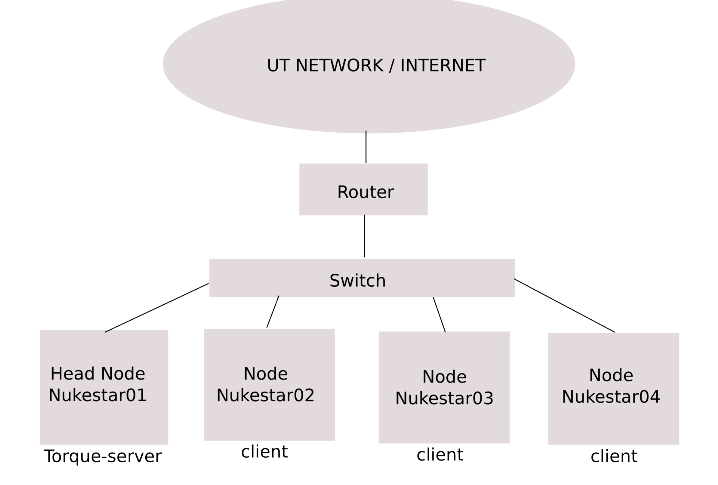
\includegraphics{nukestar.png}}\hfill}

The documentation will cover:
\begin{itemize}
\item {} 
Firewall/router setup

\item {} 
Admin Software

\item {} 
Storage node setup

\item {} 
Head node setup

\item {} 
PXE and NFS

\item {} 
Torque+maui Configuration

\item {} 
Environment Modules

\item {} 
Building software examples

\item {} 
Running jobs

\end{itemize}

The future maintainers of Nukestar should always keep security as their top priority when
setting up or modifying the cluster.  Export controlled software
will exist on the cluster.  The admin should read up on the following topics:
\begin{itemize}
\item {} 
PfSense

\item {} 
openSSH

\item {} 
groups/permissions

\end{itemize}


\chapter{Setup and Install}
\label{setup:setup-and-install}\label{setup::doc}
The pourpose of each machine in the cluster is provided below:


\section{Firewall/Router}
\label{setup:firewall-router}\begin{description}
\item[{Purpose:}] \leavevmode\begin{itemize}
\item {} 
Runs DHCP server, assigns IP adresses to all nodes in the cluster

\item {} 
Routes incomming SSH traffic to port 22 on the head node (NAT)

\item {} 
Limits the attack surface of the cluster to just ONE open port

\item {} 
Obscures the presence of the cluster on the net (inhibit portscans)

\item {} 
Logs traffic information

\end{itemize}

\item[{Firewall hardware requirements:}] \leavevmode\begin{itemize}
\item {} 
2 port 1 Gbit/sec NIC (intel prefered)

\item {} 
Modest CPU  (2 core 2GHZ+)

\item {} 
Atleast 1 GB RAM

\end{itemize}

\end{description}


\section{Head Node}
\label{setup:head-node}\begin{description}
\item[{Role:}] \leavevmode\begin{itemize}
\item {} 
Runs PBS-server and maui to distribute jobs to compute nodes

\item {} 
Raid-10 for fault tolorance operation. (\textgreater{}=4 2TB HDDs)

\item {} 
Runs NFS share

\item {} 
Contains a chroot upon which the compute node images are built

\item {} 
Runs PXE-server to distribute OS images to compute nodes on compute node bootup

\item {} 
Is the single point of entry to the cluster via ssh

\end{itemize}

\item[{Head node hardware requirements:}] \leavevmode\begin{itemize}
\item {} 
Large RAM pool (\textgreater{}=16 GB)

\item {} 
Fast CPU (8 core + Intel recommended)

\end{itemize}

\end{description}

The head node should have a VGA port so that a monitor can be connected to it.
This will ease some administrative tasks.


\section{Storage Nodes (OPTIONAL)}
\label{setup:storage-nodes-optional}\begin{description}
\item[{Role:}] \leavevmode\begin{itemize}
\item {} 
Contains storage pool(s) used as a glusterFS brick(s)

\item {} 
Runs GlusterFS-server

\item {} 
Runs NFS-server

\item {} 
Provides location to back up the Head Node's FS.

\end{itemize}

\item[{Storage node hardware:}] \leavevmode\begin{itemize}
\item {} 
Atleast 5 hard disks.  1 for OS, 4 for glusterfs/raid

\item {} 
Large RAM pool (\textgreater{}=16 GB)

\item {} 
Disks used for mass storage should be SAS 1TB+ 7200, or 10000 RPM drives

\item {} 
multi-core (4+ cores)

\end{itemize}

\end{description}


\section{Compute Nodes}
\label{setup:compute-nodes}
All large MPI tasks will be run on the compute nodes.  The PBS+maui queuing
system ensures fair utilization of the cluster's resources.
\begin{description}
\item[{Role:}] \leavevmode\begin{itemize}
\item {} 
provides computational power

\item {} 
runs pbs\_mom

\end{itemize}

\item[{Hardware:}] \leavevmode\begin{itemize}
\item {} 
many core

\item {} 
\textgreater{}= 1Gbit ethernet NiCs

\item {} 
atleast 2GB RAM/core

\end{itemize}

\end{description}


\section{Other}
\label{setup:other}\begin{description}
\item[{Network Switches:}] \leavevmode\begin{itemize}
\item {} 
at the time of this writting, dont know if ethernet or infiniband

\item {} 
provides interconnectivity between all nodes in cluster

\item {} 
Should be atleast 1Gbit/sec

\end{itemize}

\end{description}


\section{Aprox Maximum Hardware Cost}
\label{setup:aprox-maximum-hardware-cost}\begin{description}
\item[{Not including any of the bare bones computers (we got all the compute nodes for free?):}] \leavevmode\begin{itemize}
\item {} 
\$200/1TB SAS disk  x 16 = \$ 3200  for hard drives

\item {} 
\$100 for ethernet cables

\item {} 
\$2400 per 24 port infiniband switch x 2 = \$4800  (optional)

\item {} 
\$1000 for 48 infiniband cables (optional)

\item {} 
\$600 per DELL infiniband PCI card x 5 = \$3000 (optional)

\end{itemize}

\end{description}

Approx \$14200 can be spent for an optimal setup, not including cost of computational power.

\begin{notice}{note}{Note:}
The old Nukestar nodes are suitable for use as compute / storage nodes in the new cluster...
However, the old nodes lack an Infiniband interface.  It is very expensive to upgrade the old
machines to be infiniband compatible.
\end{notice}


\section{Operating System}
\label{setup:operating-system}
The operating system of choice for the cluster was chosen to be
Debian Jessie.  The authors are familiar with Debian based machines from
past experience.


\subsection{OS Install}
\label{setup:os-install}
The first task is to install the necissary operating systems on the firewall,
head node (and optionally the storage nodes).  PfSense should be installed on the Firewall.

Debian is installed on the Head node. Visit their respective websites to download bootable install isos or if
you run into issues installing either.

When installing Debian on the head node,
take care to configure the raid 10 correctly, utilizing all drives in a single mdraid storage pool.
A recommended raid 10 + LVM setup is shown below.  Logical Volume Management (LVM) is useful
when creating backup snapshots or resizing partitions online.:

\begin{Verbatim}[commandchars=\\\{\}]
\PYGZhy{}\PYGZhy{}\PYGZhy{}\PYGZhy{}\PYGZhy{}\PYGZhy{}\PYGZhy{}\PYGZhy{}\PYGZhy{}\PYGZhy{}\PYGZhy{}\PYGZhy{}\PYGZhy{}\PYGZhy{}\PYGZhy{}\PYGZhy{}\PYGZhy{}\PYGZhy{}\PYGZhy{}\PYGZhy{}\PYGZhy{}\PYGZhy{}\PYGZhy{}\PYGZhy{}\PYGZhy{}\PYGZhy{}\PYGZhy{}\PYGZhy{}\PYGZhy{}\PYGZhy{}\PYGZhy{}\PYGZhy{}\PYGZhy{}\PYGZhy{}\PYGZhy{}\PYGZhy{}\PYGZhy{}\PYGZhy{}\PYGZhy{}\PYGZhy{}\PYGZhy{}\PYGZhy{}\PYGZhy{}\PYGZhy{}\PYGZhy{}\PYGZhy{}\PYGZhy{}\PYGZhy{}\PYGZhy{}\PYGZhy{}\PYGZhy{}\PYGZhy{}\PYGZhy{}\PYGZhy{}\PYGZhy{}\PYGZhy{}\PYGZhy{}\PYGZhy{}\PYGZhy{}\PYGZhy{}\PYGZhy{}
\textbar{}                       RAID 10 Array                       \textbar{}
\textbar{} Disk 1 (sda) \textbar{} Disk 2 (sdb) \textbar{} Disk 3 (sdc) \textbar{} Disk 4 (sdd) \textbar{} \PYGZlt{}\PYGZhy{} config each divice as RAID device
\PYGZhy{}\PYGZhy{}\PYGZhy{}\PYGZhy{}\PYGZhy{}\PYGZhy{}\PYGZhy{}\PYGZhy{}\PYGZhy{}\PYGZhy{}\PYGZhy{}\PYGZhy{}\PYGZhy{}\PYGZhy{}\PYGZhy{}\PYGZhy{}\PYGZhy{}\PYGZhy{}\PYGZhy{}\PYGZhy{}\PYGZhy{}\PYGZhy{}\PYGZhy{}\PYGZhy{}\PYGZhy{}\PYGZhy{}\PYGZhy{}\PYGZhy{}\PYGZhy{}\PYGZhy{}\PYGZhy{}\PYGZhy{}\PYGZhy{}\PYGZhy{}\PYGZhy{}\PYGZhy{}\PYGZhy{}\PYGZhy{}\PYGZhy{}\PYGZhy{}\PYGZhy{}\PYGZhy{}\PYGZhy{}\PYGZhy{}\PYGZhy{}\PYGZhy{}\PYGZhy{}\PYGZhy{}\PYGZhy{}\PYGZhy{}\PYGZhy{}\PYGZhy{}\PYGZhy{}\PYGZhy{}\PYGZhy{}\PYGZhy{}\PYGZhy{}\PYGZhy{}\PYGZhy{}\PYGZhy{}\PYGZhy{}
\textbar{}                           LVM                             \textbar{} \PYGZlt{}\PYGZhy{} Use entire raid10 in LVM pool
\PYGZhy{}\PYGZhy{}\PYGZhy{}\PYGZhy{}\PYGZhy{}\PYGZhy{}\PYGZhy{}\PYGZhy{}\PYGZhy{}\PYGZhy{}\PYGZhy{}\PYGZhy{}\PYGZhy{}\PYGZhy{}\PYGZhy{}\PYGZhy{}\PYGZhy{}\PYGZhy{}\PYGZhy{}\PYGZhy{}\PYGZhy{}\PYGZhy{}\PYGZhy{}\PYGZhy{}\PYGZhy{}\PYGZhy{}\PYGZhy{}\PYGZhy{}\PYGZhy{}\PYGZhy{}\PYGZhy{}\PYGZhy{}\PYGZhy{}\PYGZhy{}\PYGZhy{}\PYGZhy{}\PYGZhy{}\PYGZhy{}\PYGZhy{}\PYGZhy{}\PYGZhy{}\PYGZhy{}\PYGZhy{}\PYGZhy{}\PYGZhy{}\PYGZhy{}\PYGZhy{}\PYGZhy{}\PYGZhy{}\PYGZhy{}\PYGZhy{}\PYGZhy{}\PYGZhy{}\PYGZhy{}\PYGZhy{}\PYGZhy{}\PYGZhy{}\PYGZhy{}\PYGZhy{}\PYGZhy{}\PYGZhy{}
\textbar{} LVM locigal vol \PYGZdq{}home\PYGZdq{}            \textbar{} LVM logical vol \PYGZdq{}root\PYGZdq{}\textbar{} \PYGZlt{}\PYGZhy{} LVM logical volumes
\PYGZhy{}\PYGZhy{}\PYGZhy{}\PYGZhy{}\PYGZhy{}\PYGZhy{}\PYGZhy{}\PYGZhy{}\PYGZhy{}\PYGZhy{}\PYGZhy{}\PYGZhy{}\PYGZhy{}\PYGZhy{}\PYGZhy{}\PYGZhy{}\PYGZhy{}\PYGZhy{}\PYGZhy{}\PYGZhy{}\PYGZhy{}\PYGZhy{}\PYGZhy{}\PYGZhy{}\PYGZhy{}\PYGZhy{}\PYGZhy{}\PYGZhy{}\PYGZhy{}\PYGZhy{}\PYGZhy{}\PYGZhy{}\PYGZhy{}\PYGZhy{}\PYGZhy{}\PYGZhy{}\PYGZhy{}\PYGZhy{}\PYGZhy{}\PYGZhy{}\PYGZhy{}\PYGZhy{}\PYGZhy{}\PYGZhy{}\PYGZhy{}\PYGZhy{}\PYGZhy{}\PYGZhy{}\PYGZhy{}\PYGZhy{}\PYGZhy{}\PYGZhy{}\PYGZhy{}\PYGZhy{}\PYGZhy{}\PYGZhy{}\PYGZhy{}\PYGZhy{}\PYGZhy{}\PYGZhy{}\PYGZhy{}
\textbar{}          /home   (\PYGZti{}1.5Tb)         \textbar{}           / (\PYGZti{}0.5Tb)  \textbar{} \PYGZlt{}\PYGZhy{} fs mounts
\PYGZhy{}\PYGZhy{}\PYGZhy{}\PYGZhy{}\PYGZhy{}\PYGZhy{}\PYGZhy{}\PYGZhy{}\PYGZhy{}\PYGZhy{}\PYGZhy{}\PYGZhy{}\PYGZhy{}\PYGZhy{}\PYGZhy{}\PYGZhy{}\PYGZhy{}\PYGZhy{}\PYGZhy{}\PYGZhy{}\PYGZhy{}\PYGZhy{}\PYGZhy{}\PYGZhy{}\PYGZhy{}\PYGZhy{}\PYGZhy{}\PYGZhy{}\PYGZhy{}\PYGZhy{}\PYGZhy{}\PYGZhy{}\PYGZhy{}\PYGZhy{}\PYGZhy{}\PYGZhy{}\PYGZhy{}\PYGZhy{}\PYGZhy{}\PYGZhy{}\PYGZhy{}\PYGZhy{}\PYGZhy{}\PYGZhy{}\PYGZhy{}\PYGZhy{}\PYGZhy{}\PYGZhy{}\PYGZhy{}\PYGZhy{}\PYGZhy{}\PYGZhy{}\PYGZhy{}\PYGZhy{}\PYGZhy{}\PYGZhy{}\PYGZhy{}\PYGZhy{}\PYGZhy{}\PYGZhy{}\PYGZhy{}
\end{Verbatim}

\begin{notice}{note}{Note:}
Ensure to mark \_atleast\_ one disk with a ``bootable'' flag durring the partitioning step.
As of the time of this writing (fall 2015) grub can boot from the /boot directory located
inside a raid 10 array.  No need to make a seperate /boot partition.
\end{notice}

The Debian installations will ask
for a new user to be setup  (in addition to the root account).  This user should be the default
system administration account.

\begin{notice}{note}{Note:}
The administrators account is NOT the root account.  We will dissallow root login from the
outside world to the cluster in future steps.  When first logging in as an admin
you must switch users to the root account to make modifications
to the base system.  Installing sudo and adding admin users to the sudo group aliviates some
minor annoyances of having to type ``su'' all the time.
\end{notice}

Durring the install procedure, there will be an option to install some software packages.  They are
all optional, however, it is recommended to install the ssh package and disable any ``printer'' packages.
It is not neccisary to install a graphical desktop environment - it will only consume hard drive space but has no
other consequences.

From here on, every command that is
executed as root will have a \code{\#} symbol preceeding it.  Every command that is executed
by a limited privilage account will be preceeded by a \code{\$}.

If no graphical desktop environment package was selected durring the initial instal, you can choose to install a minimal
gui desktop environment after you boot the new head node OS for the first time.
X11, a basic web browser such as Madori and a simple destop environment should be installed on the head node.

\begin{Verbatim}[commandchars=\\\{\}]
\PYG{c}{\PYGZsh{} apt\PYGZhy{}get update}
\PYG{c}{\PYGZsh{} apt\PYGZhy{}get install Xorg madori dwm}
\end{Verbatim}

If dwm is installed, the contensts of \code{\$\textasciitilde{}/.xinitrc} should contain.

\begin{Verbatim}[commandchars=\\\{\}]
exec dwm \PYGZam{}
\end{Verbatim}

The graphical environment is lauched by

\begin{Verbatim}[commandchars=\\\{\}]
\PYGZdl{}startx
\end{Verbatim}

This will allow easy graphical configuration of the Firewall in the following steps. Avoid running X11 as root. The
user should learn the basic commands of dwm before use.  Dwm is a minimal desktop window manager.  Read Dwm's documentation
for details on how to resize windows, open a terminal (super + enter), or launch applications (super + p or super + space by default).

\begin{notice}{note}{Note:}
It is not known at this time if infiniband will be useded for interconnects or not.  It may be very expensive
to buy the networking equipment to do so.  IF you are so lucky to have infiniband interconnects you should install
IPoIB (IP over Infiniband) on the head node and storage nodes.  This will allow the infiniband LAN to
be managed just like an ethernet network.
\end{notice}


\chapter{Configuring The Firewall/Router}
\label{firewall:configuring-the-firewall-router}\label{firewall::doc}
Configure the WAN and LAN interfaces during the initial install procedure.
Ensure a DHCP server is running on the LAN interface.  The internal network should be
setup assign IPs by default on 192.168.1.xxx/255.255.255.0 subnet.  The default IP of the LAN interface
should be 192.168.1.1.  The web configuration may be accessed at this address from the internal
network.  From the head node, type in this IP address into the web browsers URL field to do so.

The system administrator must gather all MAC addresses for all computers in the
cluster. The easiest way to do this is just to power on every computer in the cluster.  Under the
``DHCP server'' tab in the web configurator there should be information on the current DHCP leases.
This list will contain the IP addresses and MAC addresses of all computers that are currently on
the LAN network.  The easiest way to ensure the compute nodes are assigned hostnames in a physically
meaningful way is to power on each node in the cluster one-by-one, making note of it's physical location
and assigning an IP and hostname in an organized manner.

Static IP's may be assigned to all nodes in the cluster under the DHCP/LAN tab in the firewall
web-configurator once the MAC addresses of the machines are known.  Assigning each machine a static IP on
the LAN is essential to ensure that PXE booting, NFS filesystem sharing, and Torque-Maui operate properly.


\section{NAT}
\label{firewall:nat}
Stands for Network address Translation.  Under the ``NAT'' tab, configure WAN port 22 to be forwarded to the Head node.
A new firewall rule will be created.  One that allows all outside traffic targeted at port 22
to the head node port 22.  Port 22 is the default port that the ssh-server daemon listens on.


\section{Allow PXE booting}
\label{firewall:allow-pxe-booting}
In the DHCP server configuration tab ensure you enable network booting!  This is critical for the diskless clients to retrieve
the boot image from the head node at startup.  Check the TFTP server box.  Enable network booting.
For the server address put the head node's IP address \code{192.168.1.101} and for the filename put \code{pxelinux.0}.

\begin{notice}{note}{Note:}
This is VERY important!
\end{notice}


\section{Other Software}
\label{firewall:other-software}
The default install of PfSense is quite secure.  The default firewall rules (+ the NAT rule) will work for most situations.
Many packages are available that improve the monitoring capabilities of PfSense.  The admin should consider installing
PFblocker and Snort.  PFblocker allows the admin to easily block IPs from specific countries.  It is recommended to block all of
Africa, Asia + Russia, and South America.  Snort is an intrusion detection package.  You can download ``rules'' from \textless{}website here\textgreater{}
to filter and log specific traffic.


\chapter{Configure Head Node}
\label{head_node:configure-head-node}\label{head_node::doc}
Become root on the head node

\begin{Verbatim}[commandchars=\\\{\}]
su \PYGZhy{}
\end{Verbatim}

Update \code{/etc/hosts}.  Ensure this file contains all IPs and hostnames of all nodes

\begin{Verbatim}[commandchars=\\\{\}]
192.168.1.101  nukestar01
192.168.1.102  nukestar02
192.168.1.103  nukestar03
192.168.1.104  nukestar04
192.168.1.105  nukestar05
192.168.1.106 nukestar06
\end{Verbatim}

Install prerequisite software

\begin{Verbatim}[commandchars=\\\{\}]
\PYG{c}{\PYGZsh{}apt\PYGZhy{}get update}
\PYG{c}{\PYGZsh{}apt\PYGZhy{}get install tftpd\PYGZhy{}hpa nfs\PYGZhy{}kernel\PYGZhy{}server debootstrap syslinux ssh nfs\PYGZhy{}common pxelinux ntp}
\end{Verbatim}

Make root rsa ssh key pair

\begin{Verbatim}[commandchars=\\\{\}]
\PYG{c}{\PYGZsh{}cd /root}
\PYG{c}{\PYGZsh{}ssh\PYGZhy{}keygen \PYGZhy{}t rsa}
\end{Verbatim}

do not set a password when propted (password-less key based login will be used).


\section{Setup Chroot}
\label{head_node:setup-chroot}
Make a chroot root dir and chroot home dir.  Debootstrap install into /srv/nukeroot directory.

\begin{Verbatim}[commandchars=\\\{\}]
\PYG{c}{\PYGZsh{}mkdir /srv/nukeroot /srv/nukehome}
\PYG{c}{\PYGZsh{}debootstrap jessie /srv/nukeroot http://http.debian.net/debian}
\end{Verbatim}


\section{Configure NFS share folders}
\label{head_node:configure-nfs-share-folders}
Update \code{/etc/fstab} on host OS

\begin{Verbatim}[commandchars=\\\{\}]
\PYG{c}{\PYGZsh{}echo \PYGZdq{}/srv/nukehome /srv/nukeroot/home bind defaults,bind 0 0\PYGZdq{} \PYGZgt{}\PYGZgt{} /etc/fstab}
\PYG{c}{\PYGZsh{}echo \PYGZdq{}/dev /srv/nukeroot/dev auto bind 0 0\PYGZdq{} \PYGZgt{}\PYGZgt{} /etc/fstab}
\PYG{c}{\PYGZsh{}echo \PYGZdq{}/dev/pts /srv/nukeroot/dev/pts auto bind  0 0\PYGZdq{} \PYGZgt{}\PYGZgt{} /etc/fstab}
\PYG{c}{\PYGZsh{}mount \PYGZhy{}a}
\end{Verbatim}


\section{Configure Chroot}
\label{head_node:configure-chroot}
Place the contents of the base OS root public ssh key: \code{/root/.ssh/id\_rsa.pub}
in the chroot \code{/srv/nukeroot/root/.ssh/authorized\_keys} file.  Make the
\code{/srv/nukeroot/root/.ssh/authorized\_keys} file if it does not exist.

\begin{notice}{note}{Note:}
This is required for the Ansible scripts to work properly.  Ansible relies on communication over ssh.
If you do not want to use the ansible scripts, then ignore.
\end{notice}

Enter chroot

\begin{Verbatim}[commandchars=\\\{\}]
\PYG{c}{\PYGZsh{}chroot /srv/nukeroot}
\end{Verbatim}

All chroot commands will be preceeded with \code{\#\textgreater{}}.

Clear contents of \code{\#\textgreater{}/etc/hostname} because hostname will be obained from DHCP server.

Enable non-free package repo. Edit \code{\#\textgreater{}/etc/apt/sources.list} so it contains

\begin{Verbatim}[commandchars=\\\{\}]
deb http://http.debian.net/debian jessie main non\PYGZhy{}free
\end{Verbatim}

Install base packages in chroot environment

\begin{Verbatim}[commandchars=\\\{\}]
\PYGZsh{}\PYGZgt{}apt\PYGZhy{}get update
\PYGZsh{}\PYGZgt{}apt\PYGZhy{}get install aufs\PYGZhy{}tools nfs\PYGZhy{}client linux\PYGZhy{}image\PYGZhy{}3.16.0\PYGZhy{}4\PYGZhy{}amd64 vim ntp
          initramfs\PYGZhy{}tools locales dialog build\PYGZhy{}essential firmware\PYGZhy{}bnx2
\end{Verbatim}

\begin{notice}{note}{Note:}
the firmware-bnx2 package contains NIC drivers for the Dell blades used in the
current cluster.  You should identify which NIC drivers are needed for your perticular hardware.
It is very important to get the proper NIC drivers installed in the chroot because they will
be cooked into the iso that is distributed to the compute nodes on PXE boot.  If the proper
NIC driver is not avalible on the iso, the network interface on the compute nodes will obviously
not work and the compute nodes will fail to boot.
\end{notice}

... Note:

\begin{Verbatim}[commandchars=\\\{\}]
The linux\PYGZhy{}image package version will change depending on what version of Debian is being run.
3.16.0\PYGZhy{}4\PYGZhy{}amd64 is the version packaged with debian \PYGZdq{}jessie\PYGZdq{} (8.2).
\end{Verbatim}

Generate root ssh keys in chroot

\begin{Verbatim}[commandchars=\\\{\}]
\PYG{c}{\PYGZsh{}\PYGZgt{}cd /root}
\PYG{c}{\PYGZsh{}\PYGZgt{}ssh\PYGZhy{}keygen \PYGZhy{}t rsa}
\end{Verbatim}

Update \code{\#\textgreater{}/etc/hosts}.  Ensure this file contains all IPs and hostnames of all nodes

\begin{Verbatim}[commandchars=\\\{\}]
192.168.1.101  nukestar01
192.168.1.102  nukestar02
192.168.1.103  nukestar03
192.168.1.104  nukestar04
192.168.1.105  nukestar05
192.168.1.106 nukestar06
\end{Verbatim}

Update \code{\#\textgreater{}/etc/fstab} in chroot

\begin{Verbatim}[commandchars=\\\{\}]
\PYG{c}{\PYGZsh{}\PYGZgt{}echo \PYGZdq{}nukestar01:/srv/nukehome /home nfs noatime 0 0\PYGZdq{} \PYGZgt{}\PYGZgt{} /etc/fstab}
\end{Verbatim}

Generate locales

\begin{Verbatim}[commandchars=\\\{\}]
\PYG{c}{\PYGZsh{}\PYGZgt{}locale\PYGZhy{}gen en\PYGZus{}US.UTF\PYGZhy{}8}
\end{Verbatim}

Configure initramfs. Ensure the following lines exists in
\code{\#\textgreater{}/etc/initramfs-tools/initramfs.conf}:

\begin{Verbatim}[commandchars=\\\{\}]
\PYG{n}{BOOT}\PYG{o}{=}\PYG{n}{nfs}
\PYG{n}{DEVICE}\PYG{o}{=}\PYG{n}{eth0}
\end{Verbatim}

\begin{notice}{note}{Note:}
The  compute network device name (eth0 in this example) may be subject to change depending on a variety of
hardware factors.
\end{notice}

Create initrd image

\begin{Verbatim}[commandchars=\\\{\}]
\PYG{c}{\PYGZsh{}\PYGZgt{} mkinitramfs \PYGZhy{}o initrd.image.netboot}
\end{Verbatim}

Configure overlay file system script.  Aufs allows local changes to be
stored in ram on the diskless clients

\begin{Verbatim}[commandchars=\\\{\}]
\PYG{c}{\PYGZsh{}\PYGZgt{} echo aufs \PYGZgt{}\PYGZgt{} /etc/initramfs\PYGZhy{}tools/modules}
\PYG{c}{\PYGZsh{}\PYGZgt{} vim /etc/initramfs\PYGZhy{}tools/scripts/init\PYGZhy{}bottom/aufs}
\end{Verbatim}

Fill with the following

\begin{Verbatim}[commandchars=\\\{\}]
modprobe aufs
mkdir /ro /rw /aufs
mount \PYGZhy{}t tmpfs tmpfs /rw \PYGZhy{}o noatime,mode=0755
mount \PYGZhy{}\PYGZhy{}move \PYGZdl{}rootmnt /ro
mount \PYGZhy{}t aufs aufs /aufs \PYGZhy{}o noatime,dirs=/rw:/ro=ro
mkdir \PYGZhy{}p /aufs/rw /aufs/ro
mount \PYGZhy{}\PYGZhy{}move /ro /aufs/ro
mount \PYGZhy{}\PYGZhy{}move /rw /aufs/rw
mount \PYGZhy{}\PYGZhy{}move /aufs /root
exit 0
\end{Verbatim}

Make executable

\begin{Verbatim}[commandchars=\\\{\}]
\PYG{c}{\PYGZsh{}\PYGZgt{} chmod 777 /etc/initramfs\PYGZhy{}tools/scripts/init\PYGZhy{}bottom/aufs}
\end{Verbatim}

Update boot image

\begin{Verbatim}[commandchars=\\\{\}]
\PYG{c}{\PYGZsh{}\PYGZgt{} update\PYGZhy{}initramfs \PYGZhy{}u}
\end{Verbatim}

Set root password

\begin{Verbatim}[commandchars=\\\{\}]
\PYG{c}{\PYGZsh{}\PYGZgt{} passwd root}
\end{Verbatim}

Exit chroot

\begin{Verbatim}[commandchars=\\\{\}]
\PYG{c}{\PYGZsh{}\PYGZgt{} exit}
\end{Verbatim}

Copy contents of chroot root pub ssh key \code{/srv/nukeroot/root/.ssh/id\_rsa.pub} to the
base OS root \code{/root/.ssh/authorized\_keys} file.


\section{TFTP and PXE boot Setup}
\label{head_node:tftp-and-pxe-boot-setup}
The following image illustrates the setup we are working towards:

{\hfill\scalebox{0.700000}{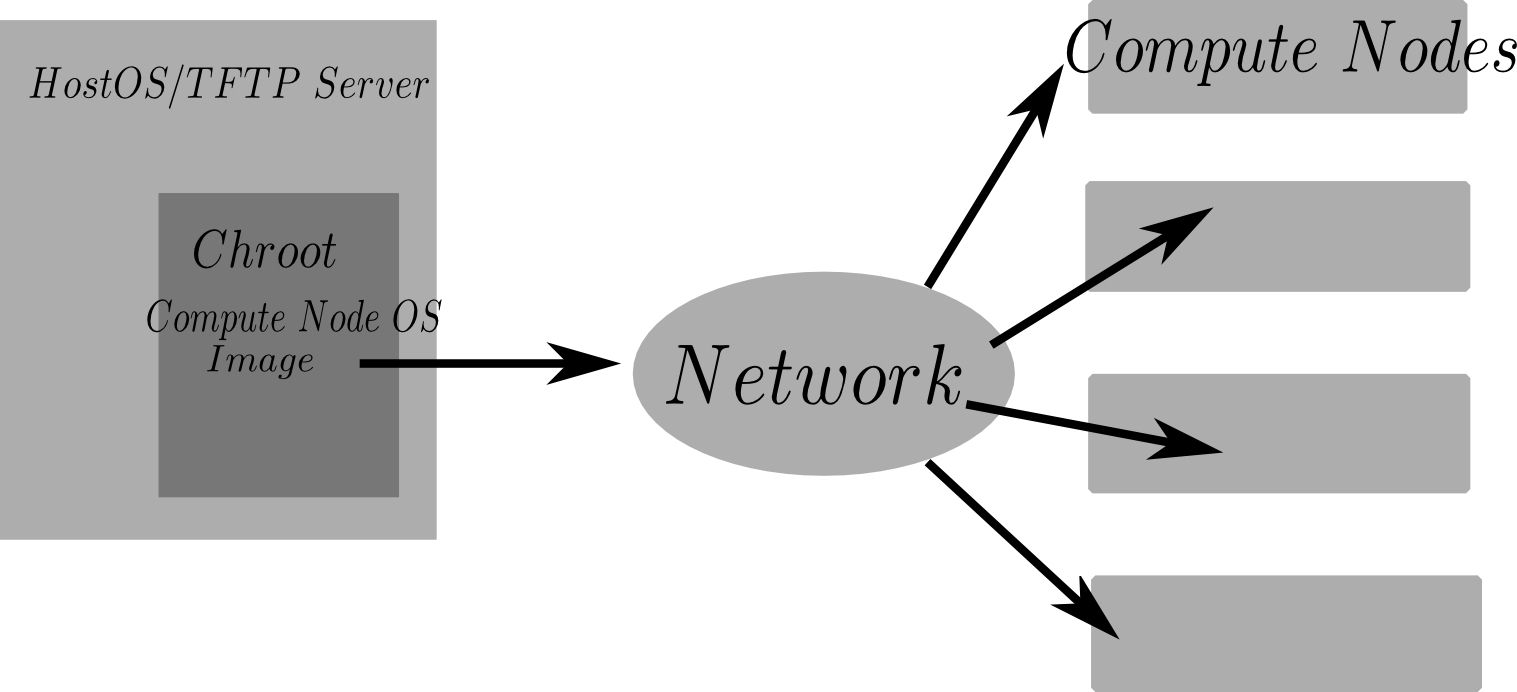
\includegraphics{nukestar_pxe.png}}\hfill}

Back on the head node copy boot image to /srv/tftp

\begin{Verbatim}[commandchars=\\\{\}]
\PYG{c}{\PYGZsh{} mkdir /srv/tftp}
\PYG{c}{\PYGZsh{} cp /srv/nukeroot/boot/initrd.img* /srv/tftp/.}
\PYG{c}{\PYGZsh{} cp /srv/nukeroot/boot/vmlinuz\PYGZhy{}* /srv/tftp/.}
\PYG{c}{\PYGZsh{} cp /usr/lib/PXELINUX/pxelinux.0 /srv/tftp/.}
\end{Verbatim}

\begin{notice}{note}{Note:}
the location of pxelinux.0 may change depending on the distribution. See specific distribution
notes on where pxelinux.0 will be placed by the syslinux or pxelinux package.
\end{notice}

Configure PXE

\begin{Verbatim}[commandchars=\\\{\}]
\PYG{c}{\PYGZsh{} mkdir /srv/tftp/pxelinux.cfg}
\end{Verbatim}

Fill \code{\#/srv/tftp/pxelinux.cfg/default} with

\begin{Verbatim}[commandchars=\\\{\}]
default Debian
prompt 1
timeout 5
label Debian
kernel vmlinuz\PYGZhy{}\PYGZlt{}name\PYGZus{}of\PYGZus{}image\PYGZgt{}
append ro initrd=initrd.img\PYGZhy{}\PYGZlt{}name\PYGZus{}of\PYGZus{}image\PYGZgt{} root=/dev/nfs ip=dhcp nfsroot=stor01:/nukeroot
\end{Verbatim}

\begin{notice}{note}{Note:}
where \textless{}name\_of\_image\textgreater{} may be something like ``3.16.0-4-amd64''.  See filename of
/srv/nukeroot/boot/vmlinuz-*
\end{notice}

Fill \code{\#/etc/default/tftpd-hpa} with the following

\begin{Verbatim}[commandchars=\\\{\}]
\PYG{n}{TFTP\PYGZus{}USERNAME} \PYG{o}{=} \PYG{l+s}{\PYGZdq{}}\PYG{l+s}{tftp}\PYG{l+s}{\PYGZdq{}}
\PYG{n}{TFTP\PYGZus{}DIRECTORY} \PYG{o}{=} \PYG{l+s}{\PYGZdq{}}\PYG{l+s}{/srv/nukeroot}\PYG{l+s}{\PYGZdq{}}
\PYG{n}{TFTP\PYGZus{}ADDRESS} \PYG{o}{=} \PYG{l+s}{\PYGZdq{}}\PYG{l+s}{0.0.0.0:69}\PYG{l+s}{\PYGZdq{}}
\PYG{n}{TFTP\PYGZus{}OPTIONS} \PYG{o}{=} \PYG{l+s}{\PYGZdq{}}\PYG{l+s}{\PYGZhy{}\PYGZhy{}secure}\PYG{l+s}{\PYGZdq{}}
\end{Verbatim}

Restart tftpd-hpa

\begin{Verbatim}[commandchars=\\\{\}]
\PYG{c}{\PYGZsh{}/etc/init.d/tftpd\PYGZhy{}hpa restart}
\end{Verbatim}

Edit \code{\#/etc/exports} file to contain NFS export details

\begin{Verbatim}[commandchars=\\\{\}]
/srv/nukeroot  192.168.1.102(ro,no\PYGZus{}root\PYGZus{}squash,async,insecure,no\PYGZus{}subtree\PYGZus{}check) \PYGZbs{}
192.168.1.103(ro,no\PYGZus{}root\PYGZus{}squash,async,insecure,no\PYGZus{}subtree\PYGZus{}check) \PYGZbs{}
192.168.1.104(ro,no\PYGZus{}root\PYGZus{}squash,async,insecure,no\PYGZus{}subtree\PYGZus{}check) \PYGZbs{}
192.168.1.105(ro,no\PYGZus{}root\PYGZus{}squash,async,insecure,no\PYGZus{}subtree\PYGZus{}check) \PYGZbs{}
192.168.1.106(ro,no\PYGZus{}root\PYGZus{}squash,async,insecure,no\PYGZus{}subtree\PYGZus{}check)
\PYGZsh{}
/srv/nukehome  192.168.1.102(rw,no\PYGZus{}root\PYGZus{}squash,async,insecure,no\PYGZus{}subtree\PYGZus{}check) \PYGZbs{}
192.168.1.103(rw,no\PYGZus{}root\PYGZus{}squash,async,insecure,no\PYGZus{}subtree\PYGZus{}check) \PYGZbs{}
192.168.1.104(rw,no\PYGZus{}root\PYGZus{}squash,async,insecure,no\PYGZus{}subtree\PYGZus{}check) \PYGZbs{}
192.168.1.105(rw,no\PYGZus{}root\PYGZus{}squash,async,insecure,no\PYGZus{}subtree\PYGZus{}check) \PYGZbs{}
192.168.1.106(rw,no\PYGZus{}root\PYGZus{}squash,async,insecure,no\PYGZus{}subtree\PYGZus{}check)
\end{Verbatim}

Run

\begin{Verbatim}[commandchars=\\\{\}]
\PYG{c}{\PYGZsh{}exportfs \PYGZhy{}ra}
\end{Verbatim}

You can now configure the compute nodes' to network boot via their bios menus.  Typically, the option to PXE (or network) boot
exists in the boot menu.  All other boot options can be disabled.  Once configured,  boot up all the compute nodes
and enjoy stateless node convinience!


\chapter{User and Group Management}
\label{user_management:user-and-group-management}\label{user_management::doc}
Cluster user permissions, ssh keys, and UID's/GID's must be managed in a very
organized way to prevent any strange permissions or connections issues down the road.
To facilitate easy user management, Ansible playbooks are provided in the repo.  Specifically,
in the /roles/common directory.  The idea is to ensure UID's, groups, and ssh keys are consistant
between the host OS and the chroot environment.


\section{Enabling Auto SSH Chroot on login}
\label{user_management:enabling-auto-ssh-chroot-on-login}
On the base system, edit \code{/etc/ssh/sshd\_config}.  At the end of this file, add

\begin{Verbatim}[commandchars=\\\{\}]
Match group users
    ChrootDirectory /srv/nukeroot
    AllowX11Forwarding yes
\end{Verbatim}

Restart sshd

\begin{Verbatim}[commandchars=\\\{\}]
\PYG{c}{\PYGZsh{}/etc/init.d/ssh restart}
\end{Verbatim}

When users in the \code{users} group ssh into the cluster, they will imediately be relegated to
the Chroot environment, where all the compute software lives.  Non-admins essentially never see the
host operating system.  It is imparitive that the admin account is not a member of the \code{users} group
so that when the admin remotely logs in, he has access to the base OS AND the chroot.  There is no good
way to break out of the chroot once you are placed inside by sshd.


\chapter{Base Software}
\label{software_setup:base-software}\label{software_setup::doc}
The software install guide is split between the host OS (base system) and the chroot environment
which is effectively the global ``compute node'' OS.

On the base system we will install:
\begin{itemize}
\item {} 
Torque+maui job scheduler

\end{itemize}

In the chroot / compute node environment, the following software will be installed:
\begin{itemize}
\item {} 
Torque (pbs\_mom)

\item {} 
gcc compilers

\item {} 
intel compiler (optional)

\item {} 
openmpi

\item {} 
environment-modules

\item {} 
user specific software

\begin{Verbatim}[commandchars=\\\{\}]
\PYGZhy{} mcnp
\PYGZhy{} python packages
\PYGZhy{} njoy
\PYGZhy{} openmc
\PYGZhy{} starccm+
\PYGZhy{} ect...
\end{Verbatim}

\end{itemize}


\section{Base OS software}
\label{software_setup:base-os-software}
Instal scripts for Torque / maui can be found in the /bash folder of this repo.


\section{Chroot / Compute Node Software}
\label{software_setup:chroot-compute-node-software}
Install the environment-modules package in chroot:

\begin{Verbatim}[commandchars=\\\{\}]
\PYG{c}{\PYGZsh{}chroot /srv/nukeroot}
\PYG{c}{\PYGZsh{}\PYGZgt{}apt\PYGZhy{}get install environment\PYGZhy{}modules}
\end{Verbatim}

run:

\begin{Verbatim}[commandchars=\\\{\}]
\PYGZdl{}\PYGZgt{}add.modules
\end{Verbatim}

For every user that wants to use environment-modules.

Then update the contents of \textasciitilde{}/.bashrc.  Uncomment the line

\begin{Verbatim}[commandchars=\\\{\}]
module() \PYGZob{} eval {}`/usr/bin/modulecmd \PYGZdl{}module\PYGZus{}shell \PYGZdl{}*{}`; \PYGZcb{}
\end{Verbatim}

and comment out any other \code{module()} definition.


\chapter{Configure Storage Nodes}
\label{storage_node:configure-storage-nodes}\label{storage_node::doc}
Configuring cluster storage precedes configuing the head node or the
compute nodes.

Here we will assume the storage node(s) have 2 drives available for both a
home and a root glusterFS brick.


\section{Setup RAID on Each Storage Node}
\label{storage_node:setup-raid-on-each-storage-node}
create a single partition on disks

\begin{Verbatim}[commandchars=\\\{\}]
\PYG{n}{fdisk} \PYG{o}{/}\PYG{n}{dev}\PYG{o}{/}\PYG{n}{sdb}
\PYG{n}{fdisk} \PYG{o}{/}\PYG{n}{dev}\PYG{o}{/}\PYG{n}{sdc}
\PYG{n}{fdisk} \PYG{o}{/}\PYG{n}{dev}\PYG{o}{/}\PYG{n}{sdd}
\PYG{n}{fdisk} \PYG{o}{/}\PYG{n}{dev}\PYG{o}{/}\PYG{n}{sde}
\end{Verbatim}

Setup RAID(s)

\begin{Verbatim}[commandchars=\\\{\}]
\PYG{n}{mdadm} \PYG{o}{\PYGZhy{}}\PYG{o}{\PYGZhy{}}\PYG{n}{create} \PYG{o}{\PYGZhy{}}\PYG{o}{\PYGZhy{}}\PYG{n}{verbose} \PYG{o}{/}\PYG{n}{dev}\PYG{o}{/}\PYG{n}{md0} \PYG{o}{\PYGZhy{}}\PYG{o}{\PYGZhy{}}\PYG{n}{level}\PYG{o}{=}\PYG{n}{mirror} \PYG{o}{\PYGZhy{}}\PYG{o}{\PYGZhy{}}\PYG{n}{raid}\PYG{o}{\PYGZhy{}}\PYG{n}{devices}\PYG{o}{=}\PYG{l+m+mi}{2} \PYG{o}{/}\PYG{n}{dev}\PYG{o}{/}\PYG{n}{sdb1} \PYG{o}{/}\PYG{n}{dev}\PYG{o}{/}\PYG{n}{sdc1}
\PYG{n}{mdadm} \PYG{o}{\PYGZhy{}}\PYG{o}{\PYGZhy{}}\PYG{n}{create} \PYG{o}{\PYGZhy{}}\PYG{o}{\PYGZhy{}}\PYG{n}{verbose} \PYG{o}{/}\PYG{n}{dev}\PYG{o}{/}\PYG{n}{md1} \PYG{o}{\PYGZhy{}}\PYG{o}{\PYGZhy{}}\PYG{n}{level}\PYG{o}{=}\PYG{n}{mirror} \PYG{o}{\PYGZhy{}}\PYG{o}{\PYGZhy{}}\PYG{n}{raid}\PYG{o}{\PYGZhy{}}\PYG{n}{devices}\PYG{o}{=}\PYG{l+m+mi}{2} \PYG{o}{/}\PYG{n}{dev}\PYG{o}{/}\PYG{n}{sdd1} \PYG{o}{/}\PYG{n}{dev}\PYG{o}{/}\PYG{n}{sde1}
\end{Verbatim}

create filesystem(s)

\begin{Verbatim}[commandchars=\\\{\}]
\PYG{n}{mkfs}\PYG{o}{.}\PYG{n}{ext4} \PYG{o}{/}\PYG{n}{dev}\PYG{o}{/}\PYG{n}{md0}
\PYG{n}{mkfs}\PYG{o}{.}\PYG{n}{ext4} \PYG{o}{/}\PYG{n}{dev}\PYG{o}{/}\PYG{n}{md1}
\end{Verbatim}

create glusterfs dir

\begin{Verbatim}[commandchars=\\\{\}]
\PYG{n}{mkdir} \PYG{o}{/}\PYG{n}{glusterfs}
\PYG{n}{mkdir} \PYG{o}{/}\PYG{n}{glusterfs}\PYG{o}{/}\PYG{n}{nukeroot}
\PYG{n}{mkdir} \PYG{o}{/}\PYG{n}{glusterfs}\PYG{o}{/}\PYG{n}{nukehome}
\end{Verbatim}

mount newly created ext4 fs to the above dirs.  Add the following to /etc/fstab

\begin{Verbatim}[commandchars=\\\{\}]
/dev/md0 /glusterfs/nukeroot ext4 defaults,noatime 0 0
/dev/md1 /glusterfs/nukehome ext4 defaults,noatime 0 0
\end{Verbatim}

run

\begin{Verbatim}[commandchars=\\\{\}]
\PYG{n}{mount} \PYG{o}{\PYGZhy{}}\PYG{n}{a}
\end{Verbatim}

Ensure that \code{/etc/hosts} contains hostnames and IPs of other storage nodes.


\section{Setup GlusterFS on Each Storage Node}
\label{storage_node:setup-glusterfs-on-each-storage-node}
Install glusterFS.

\begin{Verbatim}[commandchars=\\\{\}]
wget \PYGZhy{}O \PYGZhy{} http://download.gluster.org/pub/gluster/glusterfs/3.5/3.5.1/Debian/pubkey.gpg \textbar{} apt\PYGZhy{}key add \PYGZhy{}
echo deb http://download.gluster.org/pub/gluster/glusterfs/3.5/3.5.1/Debian/apt wheezy main \PYGZgt{}  \PYGZbs{}
              /etc/apt/sources.list.d/gluster.list
apt\PYGZhy{}get update
apt\PYGZhy{}get install glusterfs\PYGZhy{}server
\end{Verbatim}

Configure glusterFS:

\begin{Verbatim}[commandchars=\\\{\}]
gluster peer probe (hostnames of OTHER storage nodes)
\end{Verbatim}

When the above tasks have been completed on ALL storage nodes run:

Create glusterFS file system(s).  This step only needs to be performed on one of the storage nodes.

\begin{Verbatim}[commandchars=\\\{\}]
gluster volume create nukeroot replica 2 stor01:/glusterfs/nukeroot stor02:/glusterfs/nukeroot stor03:/glusterfs/nukeroot stor04:/glusterfs/nukeroot
gluster volume create nukehome replica 2 stor01:/glusterfs/nukehome stor02:/glusterfs/nukehome stor03:/glusterfs/nukehome stor04:/glusterfs/nukehome
\end{Verbatim}

Finish glusterFS install

\begin{Verbatim}[commandchars=\\\{\}]
gluster volume info
gluster volume start nukeroot
gluster volume start nukehome
\end{Verbatim}


\chapter{Indices and tables}
\label{index:indices-and-tables}\begin{itemize}
\item {} 
\DUspan{xref,std,std-ref}{genindex}

\item {} 
\DUspan{xref,std,std-ref}{modindex}

\item {} 
\DUspan{xref,std,std-ref}{search}

\end{itemize}



\renewcommand{\indexname}{Index}
\printindex
\end{document}
